\chapter{Simulator Implementation}
The integrated reinforcement learning algorithm to derive the whole schedule is driven
by a discrete event simulator. There are already some railway simulators like \textbf{OpenTrack} \cite{WEBSITE:2} and \textbf{RailML}\cite{WEBSITE:3} but they
would be useful for the final analysis of the results. Once we have the desired timetable then we can use these 
simulator softwares to determine the quality of solution. But for the implementation of the 
algorithm we have to implement the simulator on own.

\section {Railway simulator}
\subsection{Requirement}
The simulator is supposed to be robust enough that it can run both toy and real life 
examples. 
The simulator is suppose to run through several episodes during training and hence need 
to be efficient. At the
beginning of every episode, the initial locations of all the trains
are reset to their original values. It is assumed that trains that have not yet started, 
or have finished their journeys, do not
occupy any of the tracks. Following the train-to-resource mapping, 
the simulator creates a list of events for processing, one
corresponding to each train (whether already running or yet to
start its journey). Each event in the list contains the following
information: the time at which to process the event, the train to
which it corresponds, the resource where the train is currently
located, the last observed state-action pair for the train (empty
if the train is yet to start), and the direction of the train journey. 

\vspace{\baselineskip}
At each step, the algorithm moves the simulation clock to
the earliest time stamp in the event list. If multiple events are to
be processed at the same time stamp, they are handled sequentially. We are for now 
not focussing on how to avoid deadlock, but instead if we get into deadlock, we will detect and give huge
negative reward and the RL algorithm is suppose to avoid deadlock on it's own.


\subsection{Implementation}
There are two components to railway simulator :
\begin{enumerate}
    \item Underlying Railway Network. 
    \item Trains and the simulation of there movements.
\end{enumerate}

For the implementation of the railway network we can use \textbf{NetworkX}\cite{WEBSITE:4} package of python.
\textbf{NetworkX is a Python package for the creation, manipulation,
and study of the structure, dynamics, and functions of complex networks.}
\vspace{1.5cm}

Once the network is ready we have to simulate movement of each train over the network. For 
that we can use \textbf{SimPy}\cite{WEBSITE:5} package of python. \textbf{SimPy is a process-based discrete-event simulation framework based on standard Python}.
In this we can model each train as the separate process and network as the resource. We can 
model the movement of trains using this package. We yield events when the train starts from some station and once 
the train reaches the next station, event is yielded and then we can process accordingly. So whole simulation is done 
by generating events at points where the algorithm is supposed to take action.

\vspace{\baselineskip}
Once the railway network is created, train class is used to create different instances
of the trains running over the network.

% =============================================================================================================
\section{Implementation Details}

This section focuses on the implementation details of the railway simulator. Whole
implementation of railway simulator is captured by the flow diagram below. It consists of 
different modules, which in turn are made of different components. First we will have a overview of
each of the modules and its components and then move on to study them in detail. Whole code base is in 
repository \cite{WEBSITE:6}

\begin{figure}[h]
    \centering
    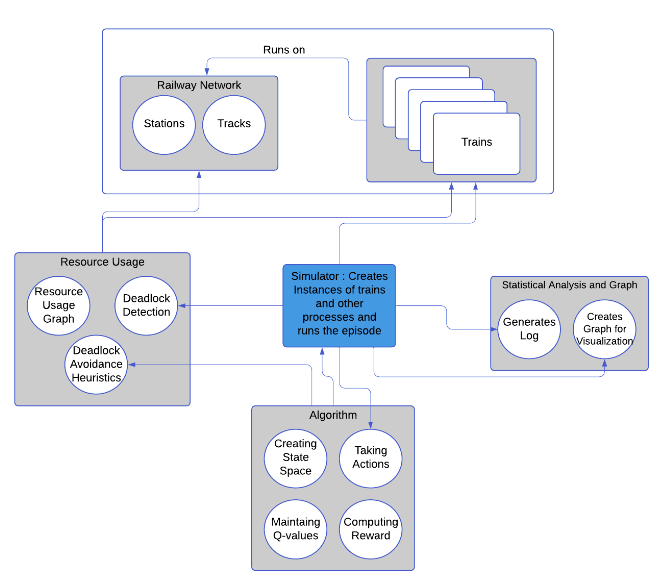
\includegraphics[width=1.0\textwidth]{Implementation}
    \caption{ Flow chart summarizing the implementation of railway simulator.  }
    \label{image-myimage1}
\end{figure}


\subsection{Modules and its components}
\begin{enumerate}
\item \textbf{Railway network and trains}

This is the main module that contains the basic architecture of railway network and the 
trains. Railway network consists of two basic components :-
\begin{itemize}
\item \textbf{Stations} : Stations in the railway network (synonymous to nodes in the network).
\item \textbf{Tracks} : Tracks connecting the stations (synonymous to edges in the network).
\end{itemize}
Once the railway network is created, train class (implemented as component) is used to create different instances
of the trains running over the network.

\item \textbf{Statistical Analysis and Graphs}

This module is responsible for creating the logs and generating necessary graphs for visualization 
and analysis.

\item \textbf{Resource Usage}

Whole railway network (station and tracks connecting the stations) is treated as pool of resource.
 Trains are ones that use this resource as they reside either on the station or the track. 
There are only fixed number of trains that can reside on the station and the track at a time.
It is also possible for the train to wait for a resource to free up, as it is occupied by other
trains. \textbf{Resource Usage Graph} component is responsible for generating the graph which show
what all resources are occupied by the trains and for what all resources train is waiting. This can be useful in detecting
deadlock.


There is another problem of deadlock which the simulator can run in. We are going to discuss this problem 
in full length in the later sections.\textbf{ Deadlock detection} and \textbf{deadlock avoidance} components
are used for detecting and avoiding the deadlock in the systems.

\item \textbf{Algorithm}

This module implements the algorithm (Q-Learning or Deep Q-learning) that helps in learning
the schedule. Currently only two components are implemented, creating state space and 
choosing action based on heuristic in \cite{ARTICLE:2}. More algorithms will be added in the future.
\vspace{2cm}
\item \textbf{Simulator}

This is one of the most important module that is responsible for creating all the processes 
that runs the simulator. It creates the environment and then invokes all the processes, then it handles 
further processing. Because of this module, we can add more modules in the future to the existing system.

\end{enumerate}

% =================================================================================================
\section{Rail Network and Train}

This module is responsible for creating the underlying railway network and the trains that run on 
these networks. Railway network module is implemented in \textbf{network.py} and train component is implemented in 
\textbf{train.py}.
\vspace{0.5cm}
\subsection {Mathematical model}
This mathematical model is from \cite{ARTICLE:2}. The railway network is modelled as a graph
$ \mathcal{G}( \mathcal{N} ,\mathcal{E})$ where $\mathcal{N}$ denotes the set of all nodes, and 
$\mathcal{E}$ denotes
the set of all edges. A set of vehicles $\mathcal{V}$ is to be scheduled
through this network, which implies that vehicles $v_i \in \mathcal{V}$
must be allotted time slots at successive nodes and edges,
such that they can move from their respective origins to
destinations via predefined routes (sequence of nodes). Each
pair of nodes is connected by at most one edge, and thus
routes also define the sequence of edges to be traversed.
Each node $n_j \in \mathcal{N}$ and edge $e_k \in \mathcal{E}$ is assumed to be
composed of one or more parallel (equivalent) resources,
denoted by $r_{m}^{nj}$ and $r_{p}^{ek}$ respectively, where $m \in \{1, \ldots R^{n}_{j}\}$
and $p \in \{1, \ldots R^{e}_{k}\}$.

\vspace{0.25cm}
Let us define the arrival time of a vehicle $v_i$ at node $n_j$ by
$t_{i}^{a} (n_j)$, and its departure time to be $t^{d}_{i} (n_j )$. Complementarily,
the arrival time to and departure time from an edge $e_k$ is
denoted by $t^{a}_{i} (e_k )$ and $t^{d}_{i} (e_k )$ respectively. If $e_k$ is traversed
upon leaving $n_j$ , then $t^{a}_{i}(e_k) = t^{d}_{i} (n_j )$. If the next node
after $e_k$ is $n_{j}^{'}$ , then $t^{d}_{i} (e_k ) = t^{a}_{i} (n_{j}^{'} )$. For simplicity, it is
assumed that all parallel resources at a node are accessible
from all resources at adjoining edges. Finally, we define the
binary variables $b^{nj}_{m}(i)$ and $b_{p}^{ek}(i)$ to be equal to 1 if $v_i$ is
allocated to resources $r_{m}^{nj}$ and $r_{p}^{ek}$ at respective nodes or
edges, and 0 otherwise. Each vehicle $v_i$ has an earliest start
time on its journey (arrival time at first node) given
by $T_i$ , and its computed finishing time (departure from last
node) is denoted by $f_i$ . Its minimum halt time at node $n_j$
is given by $H_i (n_j )$, and minimum travel time on edge $e_k$ is
given by $W_i (e_k )$.

\vspace{0.25cm}
Time constraints, $$t^{d}_{i} (n_{j} ) - t^{a}_{i} (n_{j} ) \geq H_{i} (n_{j} )$$
$$t^{d}_{i} (e_{k} ) - t^{a}_{i} (e_{k} ) \geq W_{i} (e_{k} )$$

Resource Contraints,
$$\sum_{m} b_{m}^{nj}(i) = 1$$
$$\sum_{m} b_{m}^{ek}(i) = 1$$

\subsection{Railway Network}


Railway network consists of two building blocks \textbf{Stations} and \textbf{Tracks} that connect
stations. All the fields of tracks and stations are given in the diagram below. Railway network is a weighted 
networkx graph where nodes are stations (Station class is added as attribute to the node) and edges are 
tracks running between stations (Track class is added as attribute to the edge). Input is given using two
separate text files, one corresponding to tracks and other corresponding to stations. More detailed info is 
in repository.


\begin{figure}[h]
    \centering
    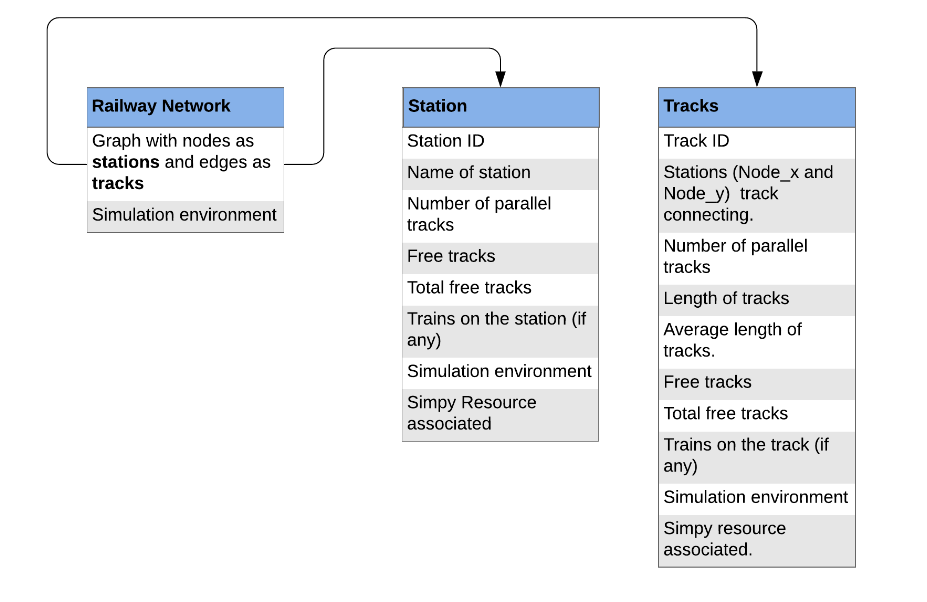
\includegraphics[width=1.0\textwidth]{Rail_train}
    \caption{ Railway Network framework }
    \label{image-myimage2}
\end{figure}

\subsection{Trains}
There are multiple trains running in the network at a time. Train class defines all the variables and methods
of this class and simulator uses this class to create process corresponding to each train (more details in simulator 
section).

\vspace{0.25cm}
Train movements over the scheduling horizon must be described in one of two ways. The first option is
to define a reference timetable which gives the desired arrival
and departure time of each train at each station. The second
option is to provide the earliest movement times from their
current locations (or origin stations), followed by the minimum
running times (on track sections between stations) and halt
times (at stations) up to the destinations. Note that the running
and halt times can be completely heterogeneous: each train
may have a different running/halt time in each resource,
depending on the length of track, the type of halt, and the
type of locomotive. The timetable can be derived by adding
the running and halt times of each train to the current time.

\begin{figure}[h]
    \centering
    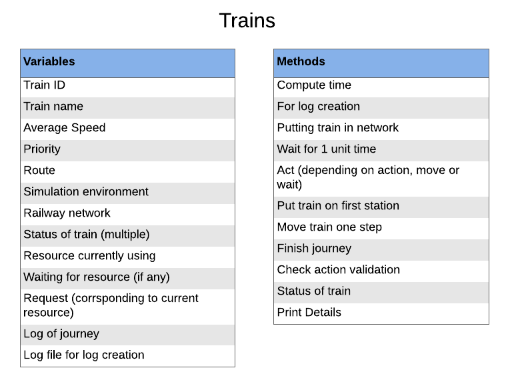
\includegraphics[width=0.8\textwidth]{train}
    \caption{ Train Variables and methods }
    \label{image-myimage3}
\end{figure}

Variables in the train class are self understood. Following are the explanation and implementation details of 
the method. For more details look into the repository where explicit documentation is given.
\begin{enumerate}
\item \textbf{Compute Time} : To calculate the travel time of the train between two stations.
\item \textbf{Log Creation} : To create log corresponding to important events for each train.
\item \textbf{Put train in network} : This method puts the train in the network and generates an event 
                                    corresponding to start time of the train. After start time, train movement is 
                                    controlled using \textbf{Act} method.
\item \textbf{Wait} : To make train wait for predefined unit of time.
\item \textbf{Act} : This method takes one argument, either to move the train or wait. Depending on the 
                    argument, specified action is taken.
\item \textbf{Put train on first station} : This method tries to put the train onto first station and thus 
                            initiating the journey of the train. It may be possible, that the station is not 
                            free, in which case the move is invalid or it waits till the resource is freed.
\item \textbf{Move train one step} : Move the train one step. If the train is on the station, then it will try to 
                                depart to the next track or if the train is on track, then it will try to arrive at the 
                                next station.
\item \textbf{Finish journey} : This method is used when the train is at the last station and it has to 
                                free the last resource.
\item \textbf{Check action validation} : Check wether the given action (move or wait) is valid for the current status of the train.
\item \textbf{Status of train} : To give the current status of the train.
\item \textbf{Print details} : To print the details of the train.
\end{enumerate}

Trains need action only for the following events :
\begin{enumerate}
\item If a train is standing at a station, the event processing time 
    corresponds to the earliest time at which the train can depart,   
    as defined by its minimum halt time at the station and by any     
    departure time constraints enforced for passenger convenience.
\item If it is running between two stations, the event processing time        
    corresponds to the earliest time at which it can arrive at the         
    next station, as defined by the length of the track and the train      
    running speed.

\item  If the train is yet to start, the event processing                      
    time is the time at which it is expected at the starting station. This event is created 
    by \textit{put train in network} method. Once this event is generated, then \textit{put train on 
    first station} is used to put the train on the first station.

\end{enumerate}


Once the train process is running, it is in one of the following states :
\begin {enumerate}
\item Train is not yet started.
\item Train is running in the network.
\item Train has reached the destination( final station in journey) but the resource is not yet freed.
\item Train has completed journey and released all the resources.
\end {enumerate}

This status is used by create statistics process, that terminates the simulation if all the trains have completed it's 
journey.




%===========================================================================================
\section{Statistical Analysis and Graph}

This module is responsible for creating the statistics and Graphs for visulalization and analysis. This 
module proves to be very important for debugging. Currently only two components are implemented but more
can be implemented in future as per the need.

\subsection{Log generatotion}
This component generates all the log in the system. There are two sets of log. One corresponding to each train that gives 
info about the status of the train at different times during the simulation. Another generates log corresponding 
to the status of the network, how many trains are there in the network and wether the network is in deadlock or not. All 
logs are generated and put in the folder \textbf{Log}.

\subsection{Graphs for visulalization}
This component creates graph for visualization, while the simulation is running. Amount of detail 
we want in the graph can be controlled using different arguments. Note that this component slows down the simulation,
so when the learning algorithm is running we can turn off this component.

\subsection{Details of the image} 
Each station is represented by node and each track is represented by edge
connecting these nodes. There can be more than one railway line on station or track, so the width of the 
nodes or the edges is directly propotional to the number of railway lines on that resource. How many lines 
are free on a given resource, that is encoded using the labels (on nodes and edges) and light green color. 
Each train running in the network is color coded. If more than 8 trains are running in the network, then all the trains
will have the same color (then image just shows the resource level information about each resource in the network).
We can control the amount of detail in the network by passing different arguments. For more details, look into the 
code repository. 


\begin{figure}[h]
    \centering
    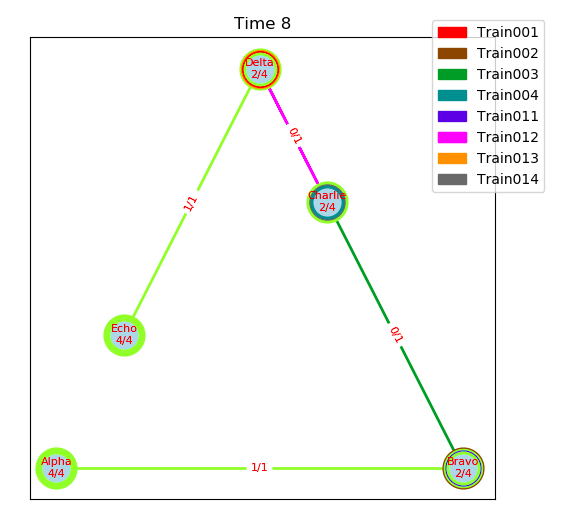
\includegraphics[width=0.5\textwidth]{graph}
    \caption{ Network with trains color coded.  }
    \label{image-myimage5}
\end{figure}

\begin{figure}[H]
    \centering
    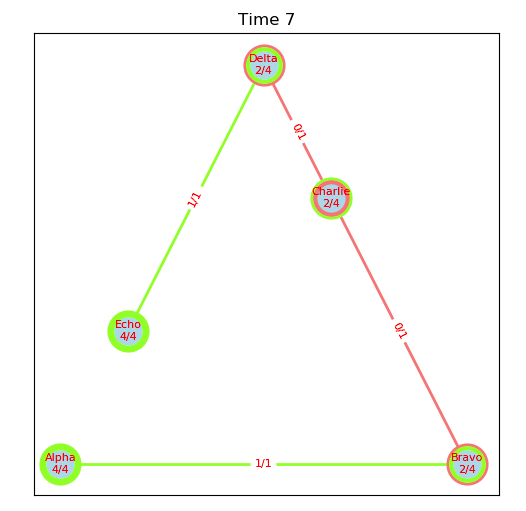
\includegraphics[width=0.5\textwidth]{graph2}
    \caption{ Network showing just what all resources are free.  }
    \label{image-myimage6}
\end{figure}

%========================================================================================
\section{Resource Usage}

This module monitors the resource usage in the network. This module is also responsible for detecting deadlock and 
implementing heuristic that avoids deadlock upto certain extent (more details in the following sections). 
  
\subsection{Resource usage graph}
This component is responsible 
for creating graph, that shows which train is using which resource(track or station) and waiting for 
which resource(if any). Pink node corresponds to train, blue corresponds to stations and green corresponds 
to track. If a train is occupying a resource (station or track), then we have an arrow from resource to train.
If a train is waiting for a resource to be freed, then we have the arrow from train to resource.

\begin{figure}[h]
    \centering
    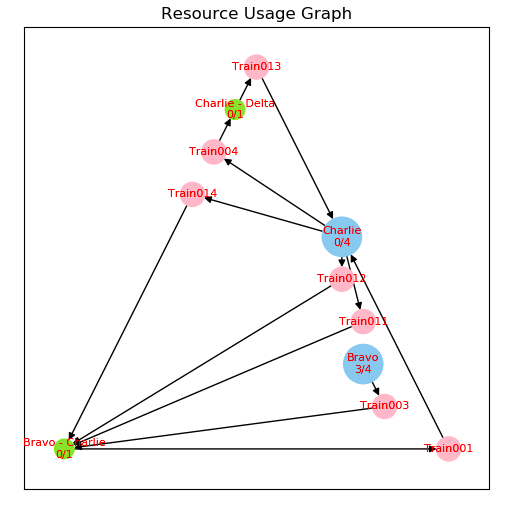
\includegraphics[width=0.65\textwidth]{resource}
    \caption{ Resource usage in the network.  }
    \label{image-myimage6}
\end{figure}

\subsection{Deadlock detection}
Simulator encounters deadlock if the next chosen move is
infeasible because $(i)$ vehicle $v$ finds all resources at the
next node occupied by other vehicles, and (ii) these other
vehicles can only release their current resources if they
move into the resource currently occupied by $v$. 
In the figure below, there are four trains at station Charlie, one train on track Delta-Charlie, trying to move to station Charlie 
and one train at track Charlie-Bravo, trying to move to station Charlie. Since no trains can move in this scenario, so it is in deadlock.

\begin{figure}[h]
    \centering
    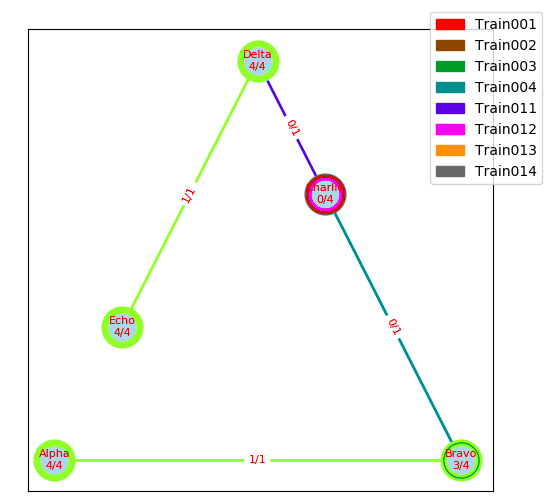
\includegraphics[width=0.65\textwidth]{deadlock}
    \caption{ Deadlock near station Charlie.  }
    \label{image-myimage6}
\end{figure}

In this simulator, each resource (station or track) is having multiple instances
(lines). If each resource have only one instance, then deadlock can be detected by cycle in resource 
usage graph. But since, each resource is having multiple instances, we have to use banker's algorithm to detect deadlock.
Once the deadlock is detected, simulation is terminated and huge negative reward is given.

\subsubsection{Banker's algorithm}

This algorithm is originally used to avoid deadlock. We are going to modify this to detect deadlock.
Here, trains are treated as processes and tracks or stations are treated as resources.
Let's $n$ be the number of processes (trains) and $m$ be the number of resource categories (number of stations and tracks in 
the network). The banker's algorithm relies on several key data structures:
\begin{enumerate}
\item $Available[m]$ indicates how many resources are currently available of each type.
\item $Max[n][m]$ indicates the maximum demand of each process of each resource.
\item $Allocation[n][m]$ indicates number of each resource category allocated to each process.
\item $Need[n][m]$ indicates the remaining resources needed of each type for each process. 
( Note that $Need[i][j] = Max[i][j] - Allocation[i][j]$   $\forall i, j$. )
\end{enumerate}

This algorithm determines if the current state of a system is safe, according to the following steps:
\begin{enumerate}
\item Let Work and Finish be vectors of length $m$ and $n$ respectively.
\begin{itemize}
\item Work is a working copy of the available resources, which will be modified during the analysis.
\item Finish is a vector of booleans indicating whether a particular process can finish (or has finished so far in the analysis).
\item Initialize Work to Available, and Finish to false for all elements.
\end{itemize}
\item Find an $i$ such that both $(A)$ $Finish[ i ] == false$, and $(B)$ $Need[i] < Work$. This process has not finished, but could with the given available working set. If no such i exists, go to step 4.
\item Set $Work = Work + Allocation[i]$, and set $Finish[i]$ to $true$. This corresponds to process $i$ finishing up and releasing its resources back 
        into the work pool. Then loop back to step 2.
\item If $finish[i] == true$  $ \forall i$, then the state is a safe state, because a safe sequence has been found.
\end{enumerate}

This algorithm is used to avoid deadlock. 
In our case $Available$ is the number of resource instances (lines 
on stations or tracks) free. $Allocated$ is the number of resource instance (lines on station or tracks) occupied 
by the train and $Requested$ is the resource instance requested by the train. 
If we use $Max = Allocated + Requested$, then above can be used to \textbf{detect deadlock} in the system.

\vspace{0.25cm}
Another important question is when to use deadlock detection algorithm. If use it very frequently 
then it's waste of computation as most the time system will not be in deadlock. If we use it very less
then system may be in deadlock for long time. So we have to find some middle ground. Here, we are currently checking deadlock
after every 20 units of time, it may be changed in the future. If the system is in deadlock, then 
simulation is terminated.

% \vspace{5cm}
\subsection{Deadlock avoidance heuristic}
Multiple trains are running in the network. It is possible that multiple trains need action at a particular simulation time.
So we have to pick one of these trains, and take action (move or wait) corresponding to 
train. This is done using deadlock avoidance heuristic based on \cite{ARTICLE:2}.
Intuitively, pick the train which is in the most
congested resource first. The lower the number of free tracks
in a resource, the higher the congestion, and the earlier the
processing of a train occupying that resource. This way we can avoid deadlock upto certain extent.

\vspace{0.25cm}
This algorithm takes TRAINS\_NEEDING\_ACTION, which is a global variable consisting of all the trains
that need action at a particular time, as input and gives the name of the train that is suitable to 
take action as output. 

\subsubsection{Algorithm}
\begin{enumerate}

\item Find status of all trains (not yet started , running , at last station or completed journey) in  
    TRAINS\_NEEDING\_ACTION.
\item Remove all trains that have completed there journey since they don't need action and generate a warning in log 
    as such train should not be in TRAINS\_NEEDING\_ACTION.
\item If there is such a train which is on last station but not freed the resource, then return that train 
     and terminate the algorithm.
\item If there is a train that has not yet started and waiting to be put on first station, then 
     return that train and terminate the algorithm.
\item Now all the trains are running. Construct an array where each element is a tuple of size 5 and corresponds to trains in 
    the TRAINS\_NEEDING\_ACTION. Items in the tuple are : 
\begin{itemize}
\item Name of the train
\item Resource (track or station) it is occupying.
\item Congestion on the resource, given by number of occupied lines on the resource.
\item Priority of the resource, given by minimum of the priority of all trains on the resource. 
\item Priority of the train
\end{itemize}

\item Pick train which is on most congested resource. If there is one such unique train then return it and 
     and terminate the algorithm. If not, go to next step.
\item Out of trains chosen from step 6, pick train on resource with highest priority. If there is one train needing action on that resource 
     then return it and terminate algorithm. If not, go to next step.
\item Out of trains chosen from step 7, pick train with highest priority. If there are multiple train then choose any one randomly and return it. 
\end{enumerate}

%============================================================================
\section{Simulator}

This module is responsible for carrying out the whole simulation and
 putting all the components in place. The way it does this is by creating
 processes that interact with each other and runs the simulation.
 This module is implemented with the help 
 of simpy that helps to create different processes. SimPy is a discrete-event simulation 
 library. The behavior of active components (like trains, deadlock detection or creating graphs) 
 is modeled with processes. All processes live in an environment. They interact with the environment 
 and with each other via events (which is created by this module). Note all the processes are 
 running \textbf{concurrently}. At last, Simpy is using priority queue to 
 order the events. There is a clock in the environment and it is the simulator that runs the clock, 
 esentially running the simulation. 

\vspace{0.25cm}

Simulator module first create the network (with the help of railway network component) and then
the \textbf{environment} under which the simulation is carried out. Then it creates 
various processes that runs in this environment. The processes are : 
\begin{enumerate}
\item \textbf{Trains}

There are multiple trains which are running in the network. Each train is an instance of 
train class implemented in the train component. Simulator creates each train as a process. These
trains are running over the same resource pool (railway network) and simulator helps in scheduling and 
running each train. Each train have two actions, either to move or to wait and these 
actions are implemented using \textbf{choose action} process.

\item \textbf{Choose action}

This process always runs and take actions for each train in the network.
Initially there are no trains in the network. Simulator puts them at the initial station at approriate time 
(depending on the schedule train is following). Once the train is put in the network, each train is either to move to the next resource
(station or track) or wait for some time at the current resource (predefined to 1 unit time, can be altered). These actions
help the train to complete it's journey from source to destination.
There can be multiple trains that need action at the same time.
TRAINS\_NEEDING\_ACTION is a global variable, that keeps track of the trains that need action at current simulation
time. So there are two tasks at hand :
\begin{itemize}
\item Choose a train from TRAINS\_NEEDING\_ACTION for taking an action. In this simulator, we are 
    using deadlock detection heuristic based on \cite{ARTICLE:2} for picking the train. Essentially this heuristic breaks
    the tie when multiple trains are waiting for taking the action.

    \item Next step is to take the action, either to move or to wait. Choice of action depends on the state
    space of the train (discussed in detail in Algorithm section). We can also randomize this process by 
    choosing the action randomly with fixed probabilities.
\end{itemize}
\item \textbf{Deadlock detection}


This process is invoked after every predefined time (20 units) and checks if the network is in deadlock 
or not.\textbf{ Banker's Algorithm} is used as the deadlock detection algorithm (discussed in detail in 
resource usage module). If the network is in deadlock, then 
simulation of the current episode terminates.

\item \textbf{Create Statistics}

This process is invoked after every predefined time (20 units) and generates statistics about the current 
state of the network in the main log file (look at log generation component). The statistics include :
\begin{itemize}
\item Number of trains not yet started. 
\item Number of trains currently running in the network.
\item Number of trains that have completed their journey but the resource is not freed.
\item Number of trains the have completed their journey and all the resources are freed.    
\end{itemize}
If all the trains have completed their journey and all resources are freed then the simulation is terminated.
More statistics about the state of the network can be added in future.  

\item \textbf{Update Graph}

This process is responsible for creating the running GIF of the railway network and the trains running on
the network. It's purpose is only visualization that further helps in debugging and analysis.
\end{enumerate}

All these processes are run by the simulator. In future, more processes can be added with different 
functionality. All one has to do is to create a component and then the simulator will create a process
that runs the component.


